% \input{"IAB/latex/TeX-Folienformat.tex"}
\input{"/Users/jonathanlatner/Google Drive/My Drive/IAB/latex/TeX-Folienformat.tex"}

\documentclass[t,8pt,utfx8]{beamer}
\usepackage{booktabs}
\usepackage{setspace}
\usepackage{parskip}
\usepackage{graphicx}
\usepackage{subcaption}
\setbeamertemplate{caption}[numbered]
\newcommand{\sprache}{\englisch}
\renewcommand{\thesubsection}{\alph{subsection})}
\usepackage[cal=pxtx, scr=dutchcal]{mathalpha}
\usepackage{forest}



\definecolor{codegreen}{rgb}{0,0.6,0}
\definecolor{codegray}{rgb}{0.5,0.5,0.5}
\definecolor{codepurple}{rgb}{0.58,0,0.82}
\definecolor{backcolour}{rgb}{0.95,0.95,0.92}


\usepackage{listings}

% Define style for R code
\lstset{
  language=R,
  basicstyle=\ttfamily\small,
  keywordstyle=\color{blue},
  stringstyle=\color{red},
  commentstyle=\color{green},
  showstringspaces=false,
  numbers=left,
  numberstyle=\tiny\color{gray},
  stepnumber=1,
  numbersep=5pt,
  breaklines=true,
  frame=single
}

\newcommand{\btVFill}{\vskip0pt plus 1filll}


\title{Buyer Beware: Understanding the trade-off between utility and risk in CART based models using simulation data}

\subtitle{
UNECE Expert Meeting on Statistical Data Collection 2025, \newline Barcelona, \newline 15-17. October, 2025}

\author{Jonathan Latner, PhD \newline Dr. Marcel Neunhoeffer \newline Prof. Dr. Jörg Drechsler}

\newcounter{noauthorlines}
\setcounter{noauthorlines}{2} % Wert für 2 Autoren über 2 Zeilen. Ggf. anpassen

% %%%%%%%%%%%%%%
% Ende Anpassung
% %%%%%%%%%%%%%%

% \input{"IAB/latex/TeX-Folienformatierung_CD_2019"}
\input{"/Users/jonathanlatner/Google Drive/My Drive/IAB/latex/TeX-Folienformatierung_CD_2019"}

% Modify the section in toc template to enumerate
\setbeamertemplate{section in toc}{%
    \inserttocsectionnumber.~\inserttocsection\par
}

% use for subsections
% \setbeamertemplate{subsection in toc}{}
\setbeamertemplate{subsection in toc}{%
    \setlength{\parskip}{1mm}
        \hskip2mm -- \hskip1mm\inserttocsubsection\par
}


\usepackage{colortbl}
\definecolor{lightgray}{gray}{0.9}

\usepackage{listings} %include R code
\lstdefinestyle{mystyle}{
    backgroundcolor=\color{backcolour},   
    commentstyle=\color{codegreen},
    keywordstyle=\color{magenta},
    numberstyle=\tiny\color{codegray},
    stringstyle=\color{codepurple},
    basicstyle=\ttfamily\tiny,
    breakatwhitespace=false,         
    breaklines=true,                 
    captionpos=b,                    
    keepspaces=true,                 
    numbers=left,                    
    numbersep=5pt,                  
    showspaces=false,                
    showstringspaces=false,
    showtabs=false,                 
    columns=fullflexible,
    frame=single,
    tabsize=2
}
\lstset{style=mystyle}


\begin{document}


\frame[plain]{\titlepage}

\begin{spacing}{1.25}

%%%%%%%%%%%%%%%%%%%%%%%%%%%%%%%%%%%%%%%%
%%%%%%%%%%%%%%%%%%%%%%%%%%%%%%%%%%%%%%%%
\section{Introduction}\label{sec:introduction}
%%%%%%%%%%%%%%%%%%%%%%%%%%%%%%%%%%%%%%%%
%%%%%%%%%%%%%%%%%%%%%%%%%%%%%%%%%%%%%%%%

\begin{frame}[c,plain]
\vskip-4mm
\begin{beamercolorbox}[wd=\boxwidth,ht=22.11mm]{transparent}%
    \vfill%
    \usebeamerfont{title}%
    \leftinsert%
    \MakeUppercase{Section \ref{sec:introduction}: Background
} % <- Hier die Überschrift eintragen
\end{beamercolorbox}
\vskip-3mm
\pgfuseimage{rahmenlinie}
\end{frame}

\begin{frame}{Overview}
\scalebox{1}{\begin{minipage}{\textwidth}
\begin{itemize}
    \item Background:
    \begin{itemize}
        \item Synthetic data are increasingly used to share data while preserving privacy.
        \item Numerous synthetic data generators (SDGs) using variety of methods
        \item CART-based SDGs: high statistical utility with high privacy risk (Little et al., 2025; Fossing, 2024; Dankar and Ibrahim, 2021)
    \end{itemize}
    \item Research question:
    \begin{itemize}
        \item If that is true, how would we know?  
        \item Do common privacy measures capture disclosure risk in synthetic data generated by CART models?
    \end{itemize}
    \item Evaluate 3x privacy measures:
    \begin{itemize}
        \item Identity disclosure risk
        \item Attribute disclosure risk
        \item Bayesian estimation of disclosure risk
    \end{itemize}
    \item 2x Data:
    \begin{itemize}
        \item Simulated dataset (Reiter et al., 2014 design: 1,000 obs., 4 binary vars., unique case).
        \item Public survey data: Social Diagnosis 2011 (SD2011).
    \end{itemize}
    \item Contributions: 
    \begin{enumerate}
        \item We show that CART-based models may produce synthetic data that sacrifices privacy protection for statistical utility.  
        \item Commonly used disclosure risk measures may not capture disclosure risk. 
        \item We propose some solutions for measuring disclosure risk (Bayesian).  
        \item More generally, users interested in measuring privacy risk should be aware of the challenges we describe here.
    \end{enumerate}
\end{itemize}
\end{minipage}}
\end{frame}



%%%%%%%%%%%%%%%%%%%%%%%%%%%%%%%%%%%%%%%%
%%%%%%%%%%%%%%%%%%%%%%%%%%%%%%%%%%%%%%%%
\section{The data}\label{sec:data}
%%%%%%%%%%%%%%%%%%%%%%%%%%%%%%%%%%%%%%%%
%%%%%%%%%%%%%%%%%%%%%%%%%%%%%%%%%%%%%%%%

\begin{frame}[c,plain]
\vskip-4mm
\begin{beamercolorbox}[wd=\boxwidth,ht=22.11mm]{transparent}%
    \vfill%
    \usebeamerfont{title}%
    \leftinsert%
    \MakeUppercase{Section \ref{sec:data}: Generate simulated data (original and synthetic)
} % <- Hier die Überschrift eintragen
\end{beamercolorbox}
\vskip-3mm
\pgfuseimage{rahmenlinie}
\end{frame}

\begin{frame}[t]\frametitle{Original data set: simulated data}
\begin{itemize}
    \item Borrowing from Reiter et al. (2014), we create a data set with $n=1000$ and 4 dichotomous, categorical variables. 
    \item The first 999 observations to be a random sample from a multinomial distribution for all combinations of $var1(0,1), var2(0,1), var3(0,1), var4(0,1)$ except the last one
    \item The last (1000$^{th}$) observation is ($var1=1,var2=1,var3=1,var4=1$). 
    \item The value of the simulated data is that we know there is a unique record because we created it.
\end{itemize}
\end{frame}

\begin{frame}[t]\frametitle{Synthetic data set}
\begin{itemize}
    \item Generate 1 synthetic data set from a CART-based SDG using the Synthpop package in R 
    \begin{itemize}
        \item We use the default settings and hyperparameter values and set a seed=$1237$. 
    \end{itemize}
    \item As a sensitivity test, we create 10 synthetic data sets from the original simulated data.  
\end{itemize}
\end{frame}

\begin{frame}[t]\frametitle{Compare simulated and synthetic data}
\begin{minipage}{0.48\textwidth}
    \begin{figure}
        \centering
        \caption{Frequency}
        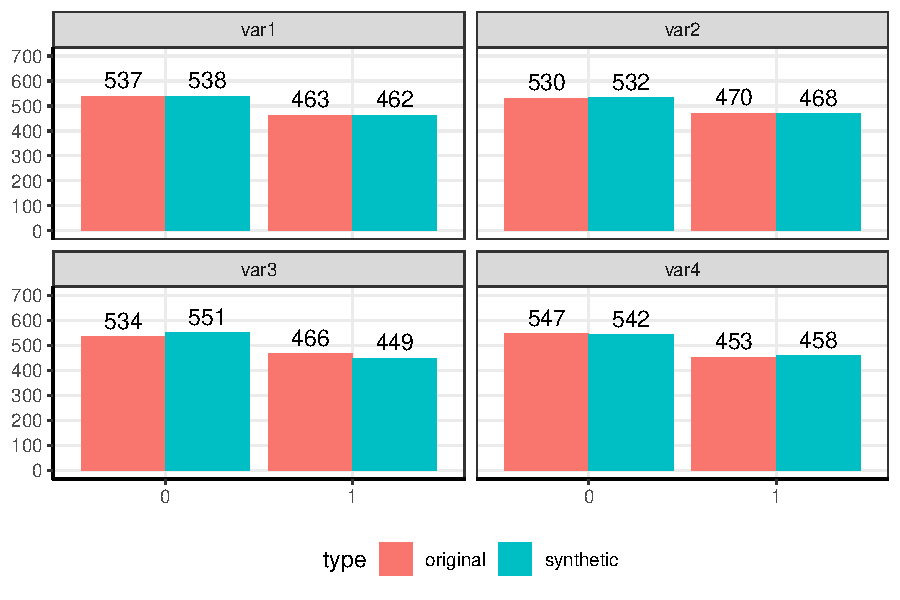
\includegraphics[width=\textwidth]{../../graphs/graph_cart_frequency_compare.pdf}
        \label{fig:frequency_compare}
    \end{figure}
\end{minipage}
\hfill
\begin{minipage}{0.48\textwidth}
    \begin{figure}
        \centering
        \caption{Histogram}
        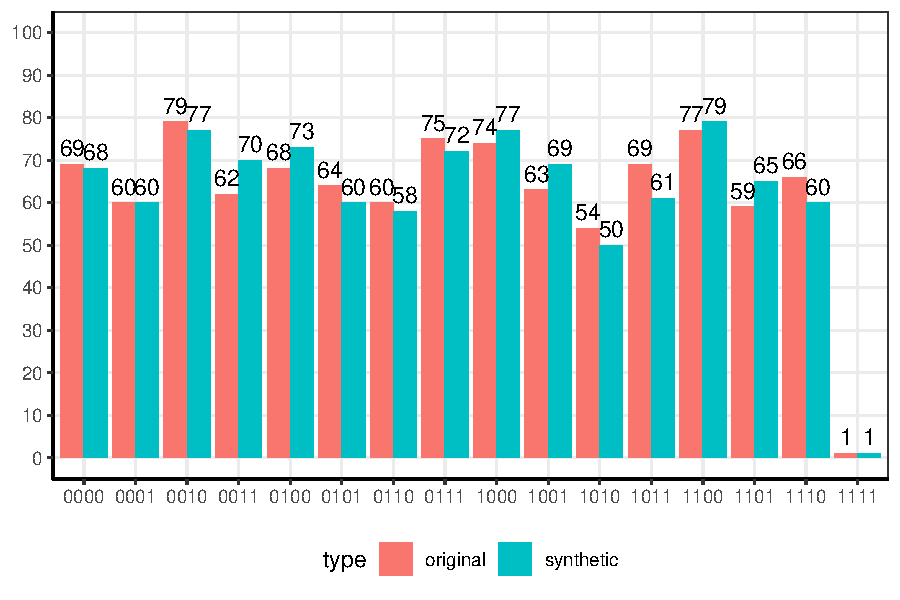
\includegraphics[width=\textwidth]{../../graphs/graph_cart_histogram_compare.pdf}
        \label{fig:histogram_compare}
    \end{figure}
\end{minipage}
\end{frame}

\begin{frame}[t]\frametitle{Compare histogram x 10 synthetic datasets}

\begin{figure}
    \caption{Multiple synthetic data sets does not reduce privacy risk}
    \resizebox{\textwidth}{!}{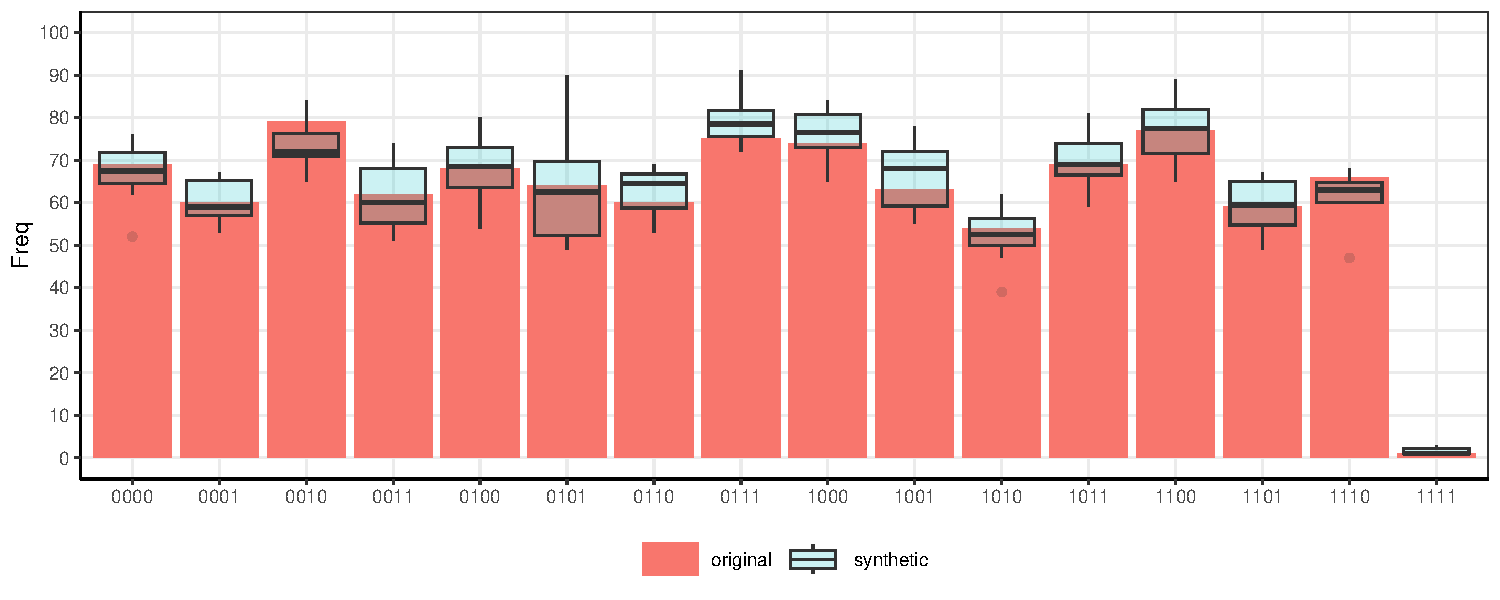
\includegraphics{../../graphs/graph_cart_histogram_compare_10_v1.pdf}}
    \label{fig:cart_histogram_compare_10}
\end{figure}

\end{frame}

\frame{\frametitle{Summary}
\begin{itemize}
    \item The problem (in our data): Synthetic data from CART models are disclosive
    \item The reason: 
    \begin{itemize}
        \item A record can only be in the synthetic data if it is also in the original data (in this simulated data).   
        \item Or the opposite: if a record is not in the original data, then it can never be in the synthetic data.
    \end{itemize}  
    \item Next section: Can an attacker identify the disclosure?
\end{itemize}
}

%%%%%%%%%%%%%%%%%%%%%%%%%%%%%%%%%%%%%%%%
%%%%%%%%%%%%%%%%%%%%%%%%%%%%%%%%%%%%%%%%
\section{The attack}\label{sec:attack}
%%%%%%%%%%%%%%%%%%%%%%%%%%%%%%%%%%%%%%%%
%%%%%%%%%%%%%%%%%%%%%%%%%%%%%%%%%%%%%%%%
\begin{frame}[c,plain]
\vskip-4mm
\begin{beamercolorbox}[wd=\boxwidth,ht=22.11mm]{transparent}%
    \vfill%
    \usebeamerfont{title}%
    \leftinsert%
    \MakeUppercase{Section \ref{sec:attack}: The attack
} % <- Hier die Überschrift eintragen
\end{beamercolorbox}
\vskip-3mm
\pgfuseimage{rahmenlinie}

\end{frame}

\frame{\frametitle{Describing the attack}
\begin{itemize}
    \item We assume a `strong' attacker similar to the attack model in differential privacy (DP). 
    \item An attacker has the following knowledge
    \begin{itemize}
        \item Knows the SDG model type (i.e. sequential CART).
        \item Knowledge of all observations in the data except the last one.  
        \item The 16 possible combinations that the last one could be.
    \end{itemize}
    \item The attacker sees the synthetic data
    \item The attacker runs the same synthetic data model (SDG) for all of the 16 different possibilities.  
    \item Then they update their beliefs about what the last record could be
\end{itemize}
}

\begin{frame}[t]\frametitle{Histogram of 16 worlds x 10 synthetic datasets}

\begin{figure}
    \caption{}
    \vskip -4mm
    \resizebox{.9\textwidth}{!}{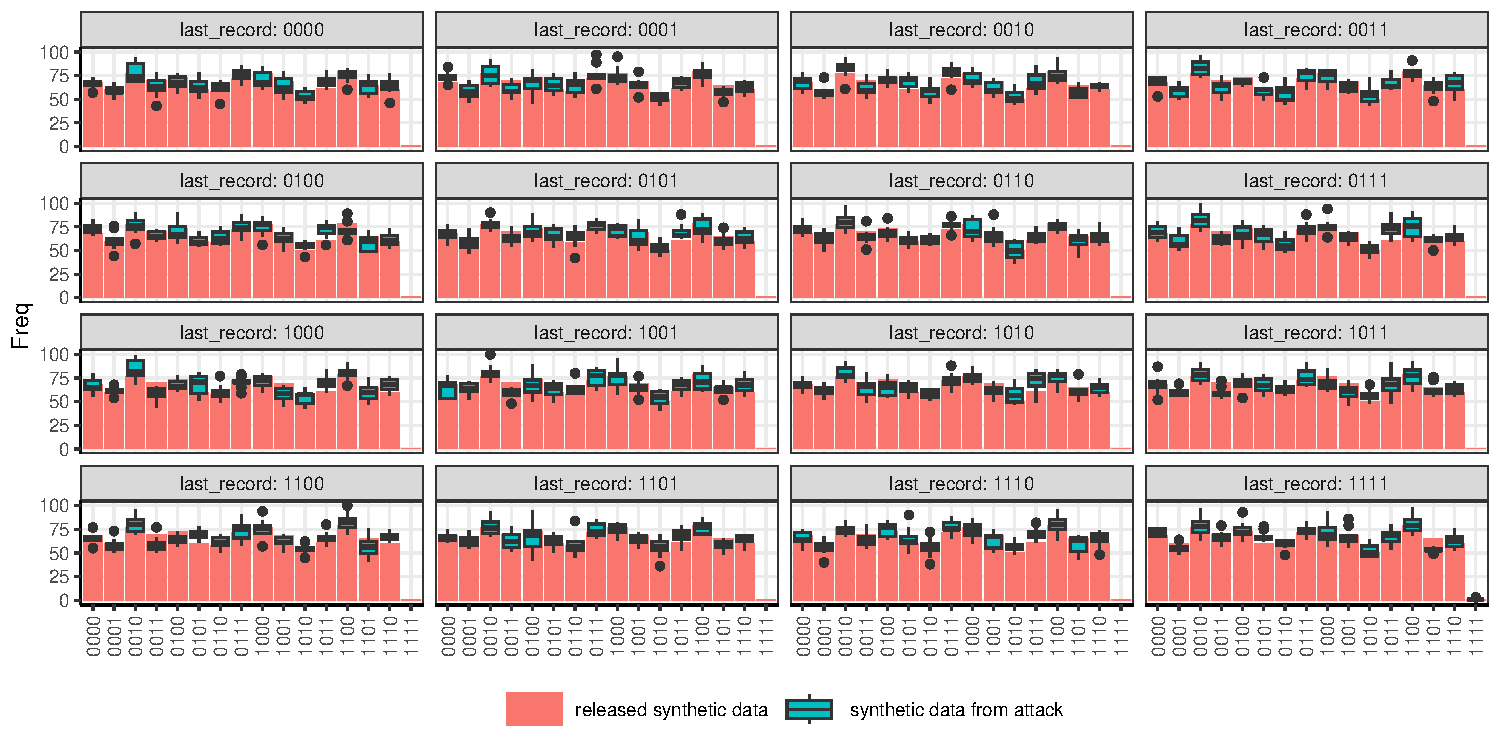
\includegraphics{../../graphs/graph_attacker_default_v1.pdf}}
    \label{fig:attacker_default}
\end{figure}


\end{frame}



\frame{\frametitle{Summary}
\begin{itemize}
    \item In our attack with our assumptions, the attacker can easily identify the last record
    \item The reason (to repeat): 
    \begin{itemize}
        \item A record can only be in the synthetic data if it is also in the original data (in this simulated data).   
        \item Or the opposite: if a record is not in the original data, then it can never be in the synthetic data.
    \end{itemize}  
    \item Next section: Can we measure this disclosure?
\end{itemize}

}


%%%%%%%%%%%%%%%%%%%%%%%%%%%%%%%%%%%%%%%%
%%%%%%%%%%%%%%%%%%%%%%%%%%%%%%%%%%%%%%%%
\section{Measuring disclosure risk}\label{sec:disclosure}
%%%%%%%%%%%%%%%%%%%%%%%%%%%%%%%%%%%%%%%%
%%%%%%%%%%%%%%%%%%%%%%%%%%%%%%%%%%%%%%%%
\begin{frame}[c,plain]
\vskip-4mm
\begin{beamercolorbox}[wd=\boxwidth,ht=22.11mm]{transparent}%
    \vfill%
    \usebeamerfont{title}%
    \leftinsert%
    \MakeUppercase{Section \ref{sec:disclosure}: Measuring disclosure risk
} % <- Hier die Überschrift eintragen
\end{beamercolorbox}
\vskip-3mm
\pgfuseimage{rahmenlinie}
\end{frame}

\begin{frame}[t]\frametitle{Three disclosure risk measures}

\begin{itemize}
    \item 2x Common disclosure risk measures reflect the current state of the art  (Raab et al., 2025)
    \begin{itemize}
        \item Identity risk ($repU$): the ability to identify individuals in the data from a set of known characteristics or `keys' ($q$).  
        \begin{itemize}
            \item  $q=var1(0,1), var2(0,1), var3(0,1)$ 
            \item Disclosure risk is how often uniqueness in the synthetic data translates into uniqueness in the original data
            \item This should be 0 because these three attributes yield $2^3 = 8$ possible combinations, none of which are unique in the dataset
        \end{itemize}
        \item Attribute risk ($DiSCO$): the ability to find out from the keys ($q$) something, not previously known or `target' ($t$)
        \begin{itemize}
            \item $t=var4(0,1)$
            \item Disclosure risk is the proportion of records in the synthetic data with the same level of $t$ for a given set of $q$
            \item This should be $>0$ because when $q=111$, there is a unique record if $t=1$. 
        \end{itemize}
    \end{itemize}
    \item 1x Alternative disclosure risk measure
    \begin{itemize}
        \item Bayesian approach (Reiter et al., 2014):   
        \begin{itemize}
            \item If posterior probability is close to the prior (e.g., uniform distribution), little or no new information is revealed.  
            \item If posterior probability is substantially larger, the intruder has learned something about the last or unique record.  
            \item In our data this should be $>0$, i.e. positive
        \end{itemize}
    \end{itemize}
\end{itemize}
\end{frame}

\begin{frame}[t]\frametitle{Results disclosure risk measures}
\begin{minipage}[t]{0.48\textwidth}
    \begin{table}[]
        \centering
        \caption{x 1 synthetic data set (seed = 1237)}
        \resizebox{\textwidth}{!}{% latex table generated in R 4.5.0 by xtable 1.8-4 package
% Wed Aug 13 15:48:17 2025
\begin{tabular}{lrrrr}
  \toprule
Data & Unique &  Identity Risk  & Attribute Risk  & Bayesian Estimate of Risk \\ 
 & & ($repU$) & ($DiSCO$) & \\
  \midrule
Original & 1&  0.00 & 0.00 &  1.00 \\ 
  Synthetic & 1& 0.00 & 0.00 & 1.00 \\ 
   \bottomrule
\end{tabular}
}
        \label{table:disclosure_risk_1}
    \end{table}

\begin{itemize}
    \small
    \item $DiSCO > 0$ only when $t$ is constant within the set of records sharing the same $q$


    \item If there is at least one unique record in the synthetic data, then there is no attribute disclosure risk because there are 2 values of $t$ within $q$ (0,1).  
    \item At the same time, if a synthetic data set is released without the unique record, then there is an attribute disclosure risk because there is only 1 value of $t$ within $q$ (1).
\end{itemize}

\end{minipage}%
\hfill%
\begin{minipage}[t]{0.48\textwidth}
    \begin{table}[]
        \centering
        \caption{x 10 synthetic data sets}
        \rowcolors{1}{white}{lightgray}
        \resizebox{\textwidth}{!}{% latex table generated in R 4.5.0 by xtable 1.8-4 package
% Wed Aug 13 15:48:18 2025
\begin{tabular}{lrrr}
  \toprule
Data & Identity Risk ($repU$) & Attribute Risk ($DiSCO$) & Bayesian Estimate of Risk \\ 
  \midrule
Original & 0.00 & 0.00 & 1.00 \\ 
  Synthetic 1 & 0.00 & 0.00 & 1.00 \\ 
  Synthetic 2 & 0.00 & 6.60 & 0.02 \\ 
  Synthetic 3 & 0.00 & 0.00 & 1.00 \\ 
  Synthetic 4 & 0.00 & 0.00 & 1.00 \\ 
  Synthetic 5 & 0.00 & 0.00 & 1.00 \\ 
  Synthetic 6 & 0.00 & 0.00 & 1.00 \\ 
  Synthetic 7 & 0.00 & 0.00 & 1.00 \\ 
  Synthetic 8 & 0.00 & 6.60 & 0.03\\ 
  Synthetic 9 & 0.00 & 0.00 & 1.00 \\ 
  Synthetic 10 & 0.00 & 0.00 & 1.00 \\ 
  Average & 0.00 & 1.32 & - \\ 
   \bottomrule
\end{tabular}
}
        \label{table:disclosure_risk_10}
    \end{table}

    \begin{itemize}
        \small
        \item $DiSCO = 6.6$.  This is the equivalent 66/1000 ((65/1000 = var1=1,var2=2,var3=1)+(1/1000 = var1=1,var2=2,var3=1,var4=1))

    \end{itemize}
\end{minipage}
\end{frame}



\frame{\frametitle{Summary}
\begin{itemize}
    \item According to common privacy measures, CART generates synthetic data with low risk
    \item However (and this is the point): We know there is a problem (because we created it)
    \item Only Bayesian approach captures disclosure risk and uncertainty about risk
    \begin{itemize}
        \item Risk is 1 whenever at least one record equal to $(1,1,1,1)$ appears in the synthetic data. 
        \item Risk $>0$ when (1,1,1,1)  does not reappear in the synthetic data. 
    \end{itemize}

\end{itemize}
}


%%%%%%%%%%%%%%%%%%%%%%%%%%%%%%%%%%%%%%%%
%%%%%%%%%%%%%%%%%%%%%%%%%%%%%%%%%%%%%%%%
\section{Is this scenario realistic?}\label{sec:reality}
%%%%%%%%%%%%%%%%%%%%%%%%%%%%%%%%%%%%%%%%
%%%%%%%%%%%%%%%%%%%%%%%%%%%%%%%%%%%%%%%%
\begin{frame}[c,plain]
\vskip-4mm
\begin{beamercolorbox}[wd=\boxwidth,ht=22.11mm]{transparent}%
    \vfill%
    \usebeamerfont{title}%
    \leftinsert%
    \MakeUppercase{Section \ref{sec:reality}: Is this scenario realistic?
} % <- Hier die Überschrift eintragen
\end{beamercolorbox}
\vskip-3mm
\pgfuseimage{rahmenlinie}

\end{frame}

\frame{\frametitle{Real world data (SD2011)}

\begin{itemize}
    \item Following the authors of Synthpop (Raab, 2024; Raab et al., 2024), we rely on data from Social Diagnosis 2011 (SD2011).  
    \item In their paper, they generate 5 synthetic data sets to illustrate their method for measuring attribute disclosure by identifying values in the target variable \texttt{depress} from keys: \texttt{sex} \texttt{age} \texttt{region} \texttt{placesize}.  
    \item To illustrate why it is a problem to measure attribute disclosure as the set of records with constant $t$ within $q$, we set $t$ as constant for all observations in all 5 synthetic data sets.  0 was chosen because it is the most frequent value in the variable \texttt{depress} (22\% of all records).  By definition, this reduces attribute disclosure risk.  
    \item In their example, attribute risk is about 9\%. However, when we modify \texttt{depress} so that it is constant (0), the risk \emph{increased} to around 15\%.
    \item Therefore, even though we know risk declined (because we reduced it), $DiSCO$ increases.

\end{itemize}


}

\begin{frame}[t]\frametitle{Results}

\begin{table}[!h]
    \centering
    \caption{Risk measures for \texttt{depress} from keys: \texttt{sex}, \texttt{age}, \texttt{region}, \texttt{placesize} (SD2011)}
    % \rowcolors{1}{white}{lightgray}
    % latex table generated in R 4.5.0 by xtable 1.8-4 package
% Fri Sep 19 10:19:15 2025
\begin{tabular}{lrrrr}
   
\toprule & 
\multicolumn{2}{l}{Identity risk ($repU$)} &
\multicolumn{2}{l}{Attribute risk ($DiSCO$)}
\\  
 
\cmidrule(lr){2-3}
\cmidrule(lr){4-5}
 
Data & Raab et al., 2024 & Modified & Raab et al., 2024 & Modified
\\ 

\midrule
Original data & 48.38 & 48.38 & 53.30 & 53.30 \\ 
   \midrule
Synthetic 1 & 14.82 & 14.82 & 8.96 & 14.74 \\ 
  Synthetic 2 & 14.20 & 14.20 & 9.90 & 14.82 \\ 
  Synthetic 3 & 15.16 & 15.16 & 10.46 & 14.94 \\ 
  Synthetic 4 & 14.12 & 14.12 & 9.68 & 14.50 \\ 
  Synthetic 5 & 14.30 & 14.30 & 8.88 & 14.66 \\ 
   \midrule
Average & 14.52 & 14.52 & 9.58 & 14.73 \\ 
   \bottomrule \\[-1.8ex] \multicolumn{5}{p{4in}}{Note: Modified indicates that values of \texttt{depress}=0 for all records in the synthetic data} 
\end{tabular}

    \label{tab:attribute_risk_sd2011}
\end{table}



\end{frame}

\begin{frame}[t]\frametitle{Summary}

\begin{itemize}
    \item When we create synthetic data to reduce attribute disclosure risk, $DiSCO$ measure increases

    \item The package authors are aware of the problem 
    \begin{itemize}
        \item  that the $DiSCO$ measure of attribute disclosure risk can indicate a high level of risk for a target variable where a high proportion of records have one level (Raab et al., 2024).
        \item The package includes a flag to allow the user to identify values within a variable that explain most of the disclosures (\texttt{check\_1way}).
    \end{itemize}
    \item We agree, but our example illustrates that the disclosure measure increases, when it should decrease.
    \item The key point is that we show that $DiSCO$ mismeasures risk using real world data
\end{itemize}

\end{frame}


%%%%%%%%%%%%%%%%%%%%%%%%%%%%%%%%%%%%%%%%
%%%%%%%%%%%%%%%%%%%%%%%%%%%%%%%%%%%%%%%%
\section{Conclusion}\label{sec:conclusion}
%%%%%%%%%%%%%%%%%%%%%%%%%%%%%%%%%%%%%%%%
%%%%%%%%%%%%%%%%%%%%%%%%%%%%%%%%%%%%%%%%
\begin{frame}[c,plain]
\vskip-4mm
\begin{beamercolorbox}[wd=\boxwidth,ht=22.11mm]{transparent}%
    \vfill%
    \usebeamerfont{title}%
    \leftinsert%
    \MakeUppercase{Section \ref{sec:conclusion}: Conclusion} % <- Hier die Überschrift eintragen
\end{beamercolorbox}
\vskip-3mm
\pgfuseimage{rahmenlinie}
\end{frame}

\begin{frame}[t]\frametitle{Summary}

\begin{itemize}
    \item CART-based synthetic data generators reproduce original data with high utility, but offer little protection for disclosive records under default settings.  
    \item Common privacy metrics may fail to detect or even misstate disclosure risk.  
    \item Bayesian approach can be a good solution, but only in low-dimensional data
    \item Key takeaway: users must understand both how SDGs generate data and how privacy measures operate.  There is no one-size-fits-all solution.  
\end{itemize}

\end{frame}

\begin{frame}[t]\frametitle{Thank you}

Jonathan Latner: \url{jonathan.latner@iab.de} \\

Reproducible code: \url{https://github.com/jonlatner/KEM\_GAN/tree/main/latner/projects/simulation} 


\end{frame}

\end{spacing}
\end{document}

